\begin{frame}{A short review}
As we saw yesterday:
\begin{itemize}
\item<2-> Topology provides many descriptors about the `shape' of a space.
\item<3-> The one of these descriptors -- homology -- is computable, which makes it particularly useful in applications.
\item<4-> Given a topological space $T$ and a field $\mathbb{F}$, the $n$-th homology group $H_n(T;\mathbb{F})$ assigns 
\item<5-> In particular, the rank of the $n$-th homology group is called the $n$-th Betti number and is denoted
	\[
	\beta_n := \textrm{rank}(H_n(T;\mathbb{F})).
	\]
\end{itemize}
\end{frame}
%---------------------------------------------------------
\begin{frame}{A short review}
\begin{itemize}
\item The $n$-th Betti number tells us about the number of $n$-dimensional holes in a space.
	\begin{itemize}
	\item<2-> $\beta_0$ counts the number of connected components in a space.
	\item<3-> What is $\beta_0$ of the following space?\\
	\
	\begin{center}
	{\fontsize{50pt}{1pt}\selectfont \={I}}
	\end{center}
	\item<4-> $\beta_0 = 3$
	\end{itemize}
\end{itemize}
\end{frame}
%---------------------------------------------------------
\begin{frame}{A short review}
\begin{itemize}
\item The $n$-th Betti number tells us about the number of $n$-dimensional holes in a space.
	\begin{itemize}
	\item<1-> $\beta_1$ counts the number of `holes' in space.
	\item<2-> You can think of a hole as something through which you can stick you arm.
	\item<3-> What are $\beta_0$ and $\beta_1$ of the following space?
	\begin{center}
	{\fontsize{50pt}{12pt}\selectfont \"{B}}
	\end{center}	
	\item<4-> $\beta_0 = 3$ and $\beta_1 = 2$
	\end{itemize}
\end{itemize}
\end{frame}
%---------------------------------------------------------
\begin{frame}{A short review}
\begin{itemize}
\item The $n$-th Betti number tells us about the number of $n$-dimensional holes in a space.
	\begin{itemize}
	\item<2-> $\beta_2$ counts the number of voids.
	\item<3-> What is $\beta_2$ of the following space?
	\begin{center}
	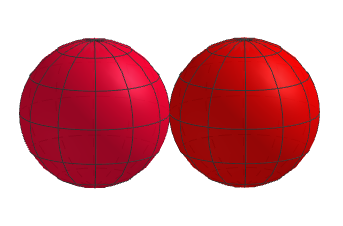
\includegraphics[scale=0.5]{images/S2VS2}
	\end{center}
	\item<4-> $\beta_2 = 2$
	\item<5-> What are $\beta_0$ and $\beta_1$?
	\item<6-> $\beta_0 = 1$ and $\beta_1 = 0$.
	\end{itemize}
\end{itemize}
\end{frame}
%---------------------------------------------------------
\begin{frame}{Persistent Homology in Dimension 0 (Clustering)}
\begin{center}
\begin{tikzpicture}[scale = 1]
    \draw plot[mark=*, mark size = 0.5, only marks] file {data/clust1.txt};
    \draw plot[mark=*, mark size = 0.5, only marks] file {data/clust2.txt};
\end{tikzpicture}
\begin{itemize}
\item<1-> Start with a set of data in a metric space. Set $r=0$.
\item<2-> Increase $r$. Create an edge between two points whenever the distance between them is less than $r$. This creates a graph.
\item<3-> The graph defines a simplicial complex.
\item<4-> If a topological property (like a Betti number) \textit{persist} over a large range of $r$, we can conclude something about the structure of the data.
\item<4-> In this case, we should expect to see $\beta_0=2$ over a large range of $r$. 
\end{itemize}
\end{center}
\end{frame}
%--------------------------------------------------------
\begin{frame}{Persistent Homology in Dimension 0 (Clustering)}
\begin{center}
\begin{tikzpicture}[scale = 1]
    \draw plot[mark=*, mark size = 0.5] file {data/clust1.txt};
    \draw plot[mark=*, mark size = 0.5] file {data/clust2.txt};
\end{tikzpicture}
\end{center}
\begin{itemize}
\item<1-> A graph similar to this should persist over a large range of $r$.
\item<2-> How could we see the clusters if these data did not lie in $\mathbb{R}^2$?
\end{itemize}
\end{frame}
%-----------------------------------------------------
\begin{frame}{RIPSER}
\begin{itemize}
\item<1-> There are several programs that do persistence.
\item<2-> We shall first look at RIPSER\cite{bauer2017ripser}.
\item<3-> Developed by Ulrich Bauer, RIPSER is a very fast C++ program for computing  Vietoris–Rips persistence barcodes.
\item<4-> Let's try this on our data with two clusters
\end{itemize}
\end{frame}
%-----------------------------------------------------
\begin{frame}{RIPSER}
\begin{center}
\begin{tikzpicture}[scale = 1]
    \draw plot[mark=*, mark size = 0.5, only marks] file {data/data1.txt};
\end{tikzpicture}
\end{center}
\begin{itemize}
\item<1-> Go to github to get the data. These data are stored as a point cloud.
\begin{center}
\footnotesize{\url{https://github.com/MatthewZabka/TDAintro.git}}
\end{center}
\item<2-> Input \texttt{data1.txt} into RISPER
\begin{center}
\url{https://live.ripser.org/}
\end{center}
\end{itemize}
\end{frame}
%------------------------------------------------------
\begin{frame}{Persistent Homology in Dimension 1}
\begin{itemize}
\item<1-> Suppose we have data that lie on the circle.
\begin{center}
\begin{figure}
\begin{tikzpicture}[scale = 1.5]
    \draw plot[mark=*, mark size = 0.5, only marks] file {data/data2.txt};
\end{tikzpicture}
\caption{An unrealistic example, where data lie perfectly on $S^1$.}
\end{figure}
\end{center}
\item<2-> Input \texttt{data2.txt} into RIPSER.
\item<2-> Wait \ldots data are never this nice.
\end{itemize}
\end{frame}
%------------------------------------------------------
\begin{frame}{Persistent Homology in Dimension 1}
\begin{itemize}
\item<1-> Suppose we have data that \textbf{almost} lie on the circle.
\begin{center}
\begin{figure}
\begin{tikzpicture}[scale = 1.5]
    \draw plot[mark=*, mark size = 0.5, only marks] file {data/data3.txt};
\end{tikzpicture}
\caption{A slightly more realistic example.}
\end{figure}
\end{center}
\item<2-> Input \texttt{data3.txt} into RIPSER.
\end{itemize}
\end{frame}